
\begin{center}
\includegraphics[width=7cm]{python_codes/fieldstone_41/images/setup}
\end{center}

Original experiment: domain is $0.9142\times1$, viscosity is $\eta=100$, 
densities are 1000 and 1010 (i.e. $\delta \rho=10$).
Our domaini is $9142\times10000$m, our viscosity is $\eta=10^{19}$,
our densities are 2150 and 2600, i.e. $\delta\rho = 450$.
In both we set g=10.

In the original paper, 
length=1, viscosity=100, gravity =10, density contrast =10 and time unit =1,
so the dimensionless quantity
\[
\frac{\eta}{\delta\rho \cdot g \; length \cdot time} = \frac{100}{10 \cdot 10 \cdot 1 \cdot 1} =1
\]
If we now run a geometrically similar experiment with 
length=10km, viscosity=$10^{19}$, gravity=10, density contrast=450 and time unit = $t$
then we should also have 
\[
\frac{\eta}{\delta\rho \cdot g \; length \cdot time} = \frac{10^{19}}{450 \cdot 10 \cdot 10^4 \cdot t} =1
\]
i.e.,
\[
t = \frac{10^{14}}{450} \simeq 2.222 \cdot 10^{11}\text{s}
\]
This means that in order to plot our results against those in van Keken et al, their results
must be scaled: times must be multiplied by $t$ and velocities divided/multiplied (??) by 
$t/length = 2.222 \cdot 10^{7}\text{m/s}$  

Describe here marker to node projection. Q1 projection onto nodes, then 
shape functions used to bring density to quadrature points. 


Simulations end when an element does not contain any particle.
\begin{center}
\includegraphics[width=7cm]{python_codes/fieldstone_41/results/vrms.pdf}
\includegraphics[width=7cm]{python_codes/fieldstone_41/results/mass.pdf}\\
\includegraphics[width=7cm]{python_codes/fieldstone_41/results/nmarker.pdf}
\end{center}

\begin{center}
\includegraphics[width=5cm]{python_codes/fieldstone_41/results/64x64_10_RK3/markers0000}
\includegraphics[width=5cm]{python_codes/fieldstone_41/results/64x64_10_RK3/markers0143}
\includegraphics[width=5cm]{python_codes/fieldstone_41/results/64x64_10_RK3/rho_nodal_0143}\\
{\captionfont 64x64 simulation right before crash}
\end{center}




